
\scalebox{1.3}{
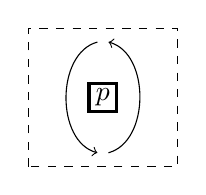
\begin{tikzpicture}{scale=2.1}

  \newcommand\X{65pt};
  \newcommand\Y{15pt};


%  \draw[->] (0*\X, 0*\Y) -- node{rejoint} (-27+1*\X, 0*\Y);


  \draw[fill=white, dashed]
  (0*\X, 0*\Y) +(-27pt,-25pt) rectangle +(27pt,25pt);

  \draw[fill=white, very thick]
  (0*\X, 0*\Y) node{$p$} +(-5pt,-5pt) rectangle +(5pt,5pt);
  
  \draw[->] (  2+0*\X, -20+0*\Y ) to[out=15,in=-15] (2+0*\X, 20+0*\Y);
  \draw[<-] ( -2+0*\X, -20+0*\Y ) to[out=165,in=-165] (-2+0*\X, 20+0*\Y);

 
\end{tikzpicture}
}